% !TEX encoding = UTF-8 Unicode
\newpage

\chapter{Matériel}
\section{Matériel utilisé}
\lettrine[lines=1]{J}'utise pour le robot, un châssis récupéré d'un robot Makebloc, 2 moteurs à courant continus, un capteur de distance à ultrasons, un gyroscope et des cartes électroniques de contrôle, un modem  Wifi, un coupleur de piles, des powerbanks.

\subsection{Le chassis}
Sur le chassis sont fixés la boite de contrôle, le modem wifi, les moteurs avec les roue, la roulette de nez.

\subsection{Les moteurs}
Il s'agit de 2 moteurs à courant continus placés de chaque côté, reliés directement aux roues.
\\Les moteurs sont pilotés par un pont en H et par modulation PWM

\subsection{Le capteur de distance}
C'est la capteur ultrason qui permet de mesurer sa distance par rapport à un obstacle
\begin{center}
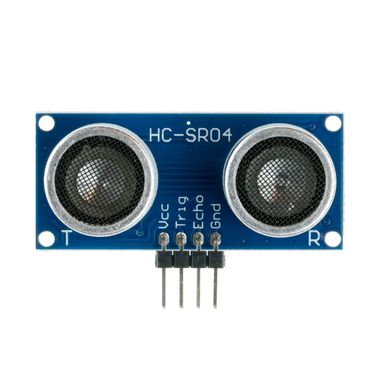
\includegraphics[width=4cm]{introduction/hrsr04.jpeg} 
\end{center}

\subsection{Le gyroscope}
Il permet de mesurer sa rotation angulaire sur les 3 axes X, Y et Z.

\subsection{La carte mère }
Il s'agit d'une carte Zybo de Digilent, équipée d'un Soc Zynq7000 ARM CortexA9 + FPGA

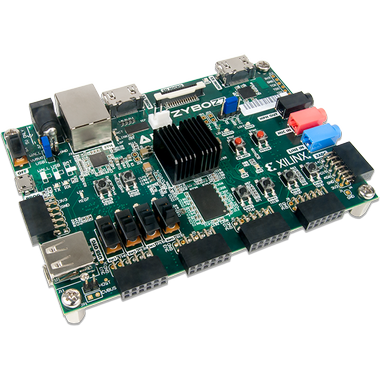
\includegraphics[width=8cm]{introduction/zybo-z7-3.png} 
\end{center}
 